\documentclass{abntex2}
\usepackage[utf8]{inputenc}
\usepackage{graphicx}
\usepackage[num]{abntex2cite}

\titulo{Experimento 1: Circuitos com diodos}
\autor{Lucas Rezende de Macedo - 14/0026363\\Jônatas Ribeiro Senna Pires - xx/xxxxxxx}
\data{31 de Março de 2018}
\local{Brasília, Distrito Federal}

\begin{document}

\imprimircapa
\imprimirfolhaderosto

\tableofcontents
\listoffigures
\clearpage

\chapter{Experiências}

O procedimento experimental consiste de verificar a diferença entre as ondas de entrada e saída dos circuitos da figura \ref{fig:circuitos} e a característica de transferência de cada circuito.

\begin{figure}[h]
  \centering
  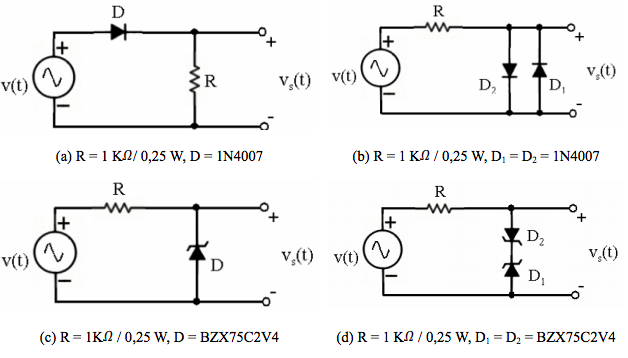
\includegraphics[width=.8\textwidth]{circuitos.png}
  \caption{Circuitos montados no procedimento experimental.}
  \label{fig:circuitos}
\end{figure}

\section{Experiência 1}

Para o circuito da figura \ref{fig:circuitos}(a) temos que a entrada ($v_I$) e saída ($v_o$) são definidas conforme a figura \ref{fig:io1} em que, no intervalo entre $x_0$ e $x_1$, o diodo $D$ encontra-se diretamente polarizado e, no intervalo $x_1$ a $x_2$, encontra-se reversamente polarizado, para esse circuito, não houve ruptura.

A característica de transferência $v_o \times v_I$ é caracterizada pela figura \ref{fig:diff1}.

\begin{figure}[h]
  \centering
  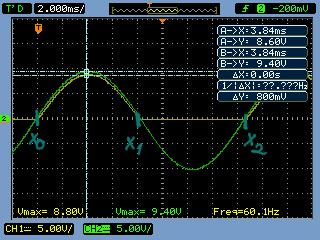
\includegraphics[width=.8\textwidth]{circuito-1a-esboco2.png}
  \caption{Gráfico da entrada (verde) e saída (amarelo) do circuito da figura \ref{fig:circuitos}(a).}
  \label{fig:io1}
\end{figure}

\begin{figure}[h]
  \centering
  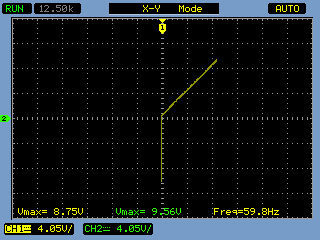
\includegraphics[width=.8\textwidth]{diferenca-1a.png}
  \caption{Gráfico da característica de transferência do circuito da figura \ref{fig:circuitos}(a) em que $v_o$ está no eixo horizontal e $v_I$ está no eixo vertical.}
  \label{fig:diff1}
\end{figure}

\section{Experiência 2}

Para o circuito da figura \ref{fig:circuitos}(b) temos que a entrada ($v_I$) e saída ($v_o$) são definidas conforme a figura \ref{fig:io2}  em que, no intervalo entre $x_0$ e $x_1$, o diodo $D_2$ encontra-se diretamente polarizado e $D_1$ encontra-se inversamente polarizado, no intervalo $x_1$ a $x_2$, $D_2$ encontra-se reversamente polarizado e $D_1$ encontra-se diretamente polarizado, para esse circuito, não houve ruptura.

A característica de transferência é caracterizada pela figura \ref{fig:diff2}.

\begin{figure}[h]
  \centering
  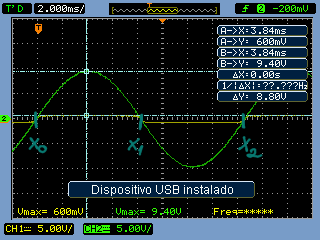
\includegraphics[width=.8\textwidth]{circuito-1b-esboco2.png}
  \caption{Gráfico da entrada (verde) e saída (amarelo) do circuito da figura \ref{fig:circuitos}(b).}
  \label{fig:io2}
\end{figure}

\begin{figure}[h]
  \centering
  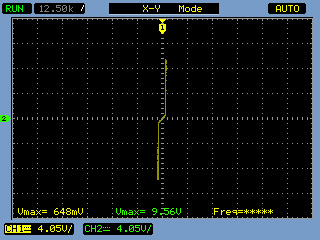
\includegraphics[width=.8\textwidth]{diferenca-1b.png}
  \caption{Gráfico da característica de transferência do circuito da figura \ref{fig:circuitos}(b) em que $v_o$ está no eixo horizontal e $v_I$ está no eixo vertical.}
  \label{fig:diff2}
\end{figure}

\section{Experiência 3}

Para o circuito da figura \ref{fig:circuitos}(c) temos que a entrada ($v_I$) e saída ($v_o$) são definidas conforme a figura \ref{fig:io3}  em que, no intervalo entre $x_0$ e $x_1$, o diodo $D$ encontra-se em ruptura, no intervalo $x_1$ a $x_2$, $D$ encontra-se diretamente polarizado, para esse circuito, houve polarização reversa em $D$ nos instantes $x_0$ e $x_2$.

A característica de transferência é caracterizada pela figura \ref{fig:diff3}.

\begin{figure}[h]
  \centering
  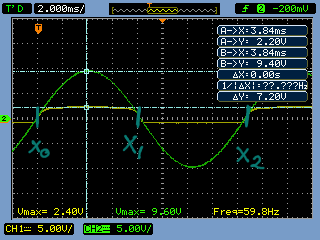
\includegraphics[width=.8\textwidth]{circuito-1c-esboco2.png}
  \caption{Gráfico da entrada (verde) e saída (amarelo) do circuito da figura \ref{fig:circuitos}(c).}
  \label{fig:io3}
\end{figure}

\begin{figure}[h]
  \centering
  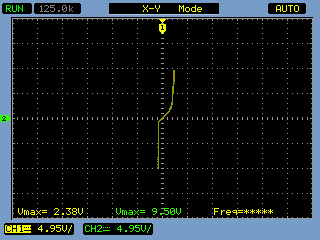
\includegraphics[width=.8\textwidth]{diferenca-1c.png}
  \caption{Gráfico da característica de transferência do circuito da figura \ref{fig:circuitos}(c) em que $v_o$ está no eixo horizontal e $v_I$ está no eixo vertical.}
  \label{fig:diff3}
\end{figure}

\section{Experiência 4}

Para o circuito da figura \ref{fig:circuitos}(d) temos que a entrada ($v_I$) e saída ($v_o$) são definidas conforme a figura \ref{fig:io4}  em que, no intervalo entre $x_0$ e $x_1$, o diodo $D_2$ encontra-se diretamente polarizado e $D_1$ encontra-se em ruptura, no intervalo $x_1$ a $x_2$, $D_2$ encontra-se em ruptura e $D_1$ encontra-se diretamente polarizado, para esse circuito, houve polarização inversa em $D_1$ nos momentos $x_0$ e $x_2$ e em $D_2$ no momento $x_1$.

A característica de transferência é caracterizada pela figura \ref{fig:diff4}.

\begin{figure}[h]
  \centering
  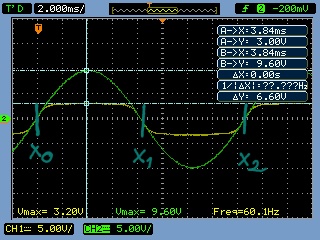
\includegraphics[width=.8\textwidth]{circuito-1d-esboco2.png}
  \caption{Gráfico da entrada (verde) e saída (amarelo) do circuito da figura \ref{fig:circuitos}(d).}
  \label{fig:io4}
\end{figure}

\begin{figure}[h]
  \centering
  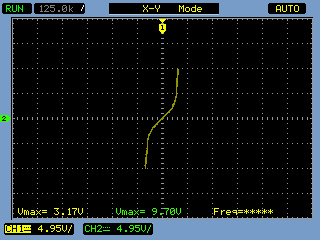
\includegraphics[width=.8\textwidth]{diferenca-1d.png}
  \caption{Gráfico da característica de transferência do circuito da figura \ref{fig:circuitos}(d) em que $v_o$ está no eixo horizontal e $v_I$ está no eixo vertical.}
  \label{fig:diff4}
\end{figure}

\chapter{Discussão}

\section{Comparação com o modelo ideal}

\section{Circuitos retificadores e limitadores}

O circuito retificador tem esse nome dado que para uma tensão menor que sua tensão de polarização direta ($V_d$), a saída torna-se uma tensão contínua, como podemos ver na figura \ref{fig:retificador}, no caso do circuito da figura \ref{fig:circuitos}(a) essa tensão de saída é 0.

O circuito limitador tem esse nome porque ele faz com que a tensão máxima que o circuito possa atingir seja seu $V_d$, como podemos ver na figura \ref{fig:limitador}.

\begin{figure}[h]
  \centering
  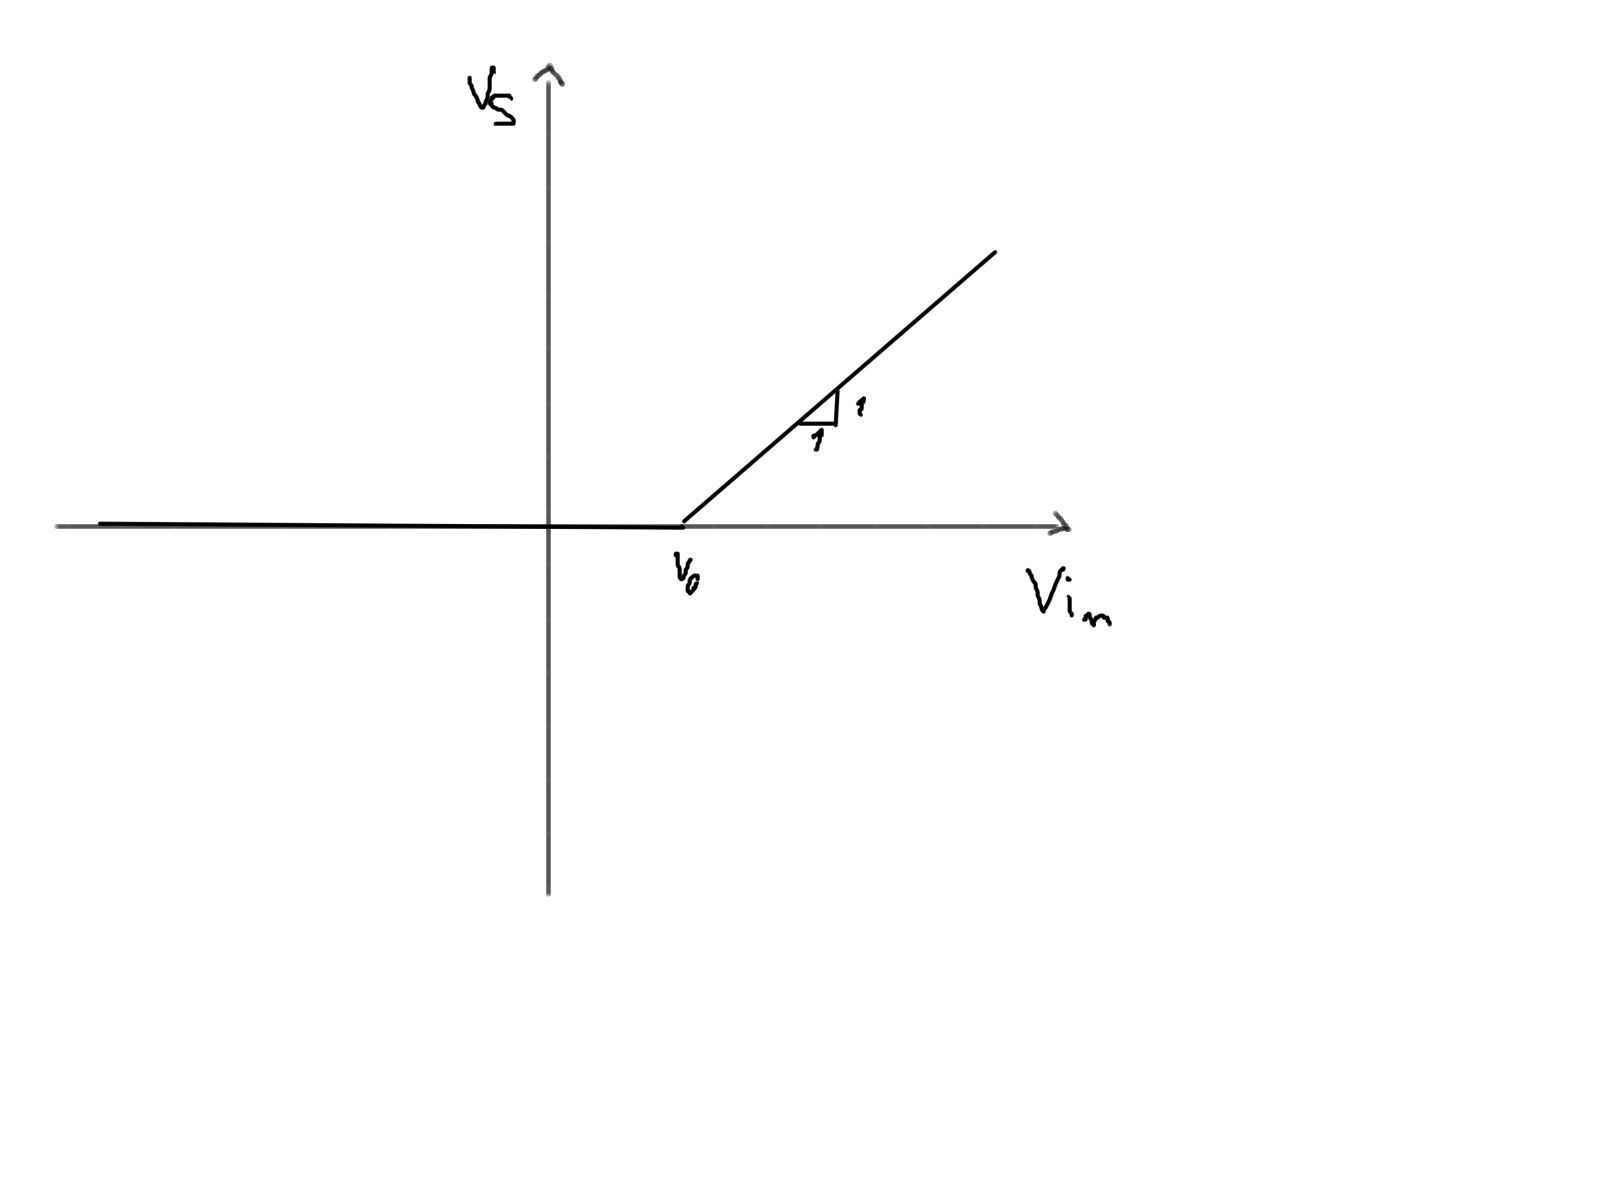
\includegraphics[width=.8\textwidth]{grafRetificador.jpeg}
  \caption{Gráfico da característica de transferência de um circuito retificador.}
  \label{fig:retificador}
\end{figure}

\begin{figure}[h]
  \centering
  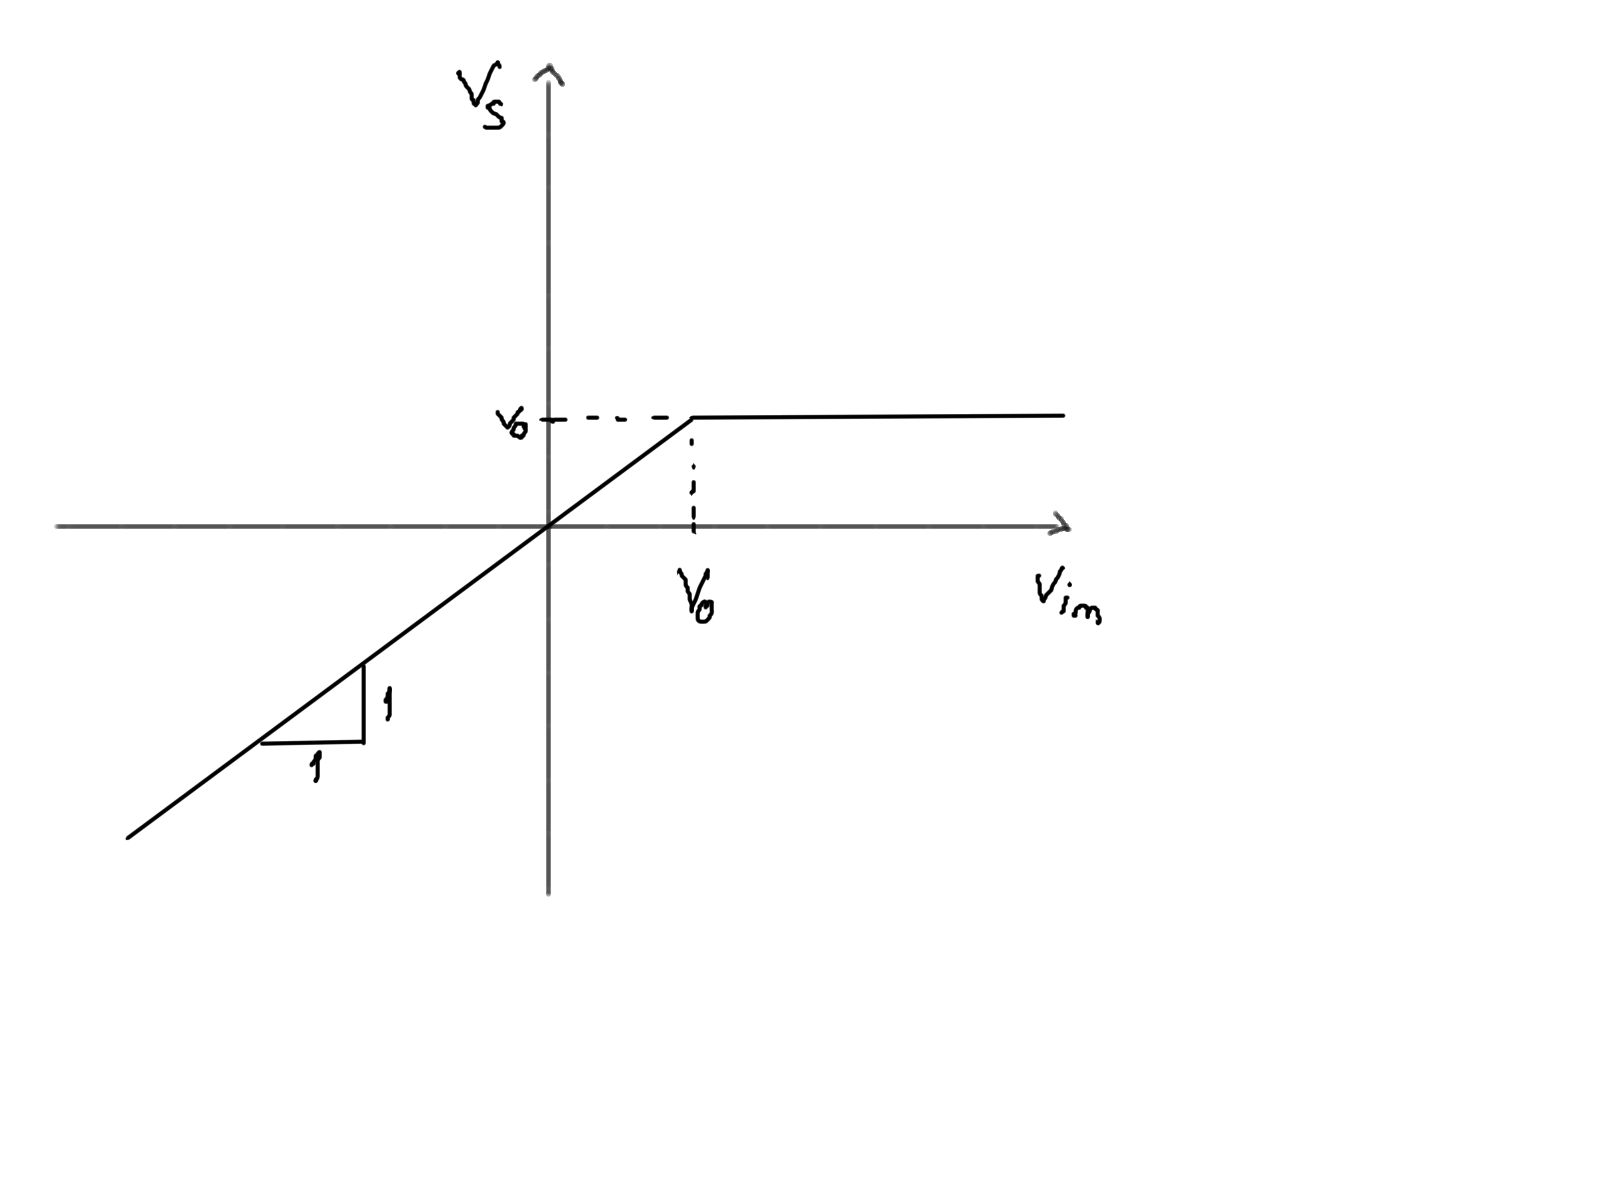
\includegraphics[width=.8\textwidth]{grafLimitador.jpg}
  \caption{Gráfico da característica de transferência de um circuito limitador.}
  \label{fig:limitador}
\end{figure}

Os circuitos da figura \ref{fig:circuitos} com exceção do circuito (a) podem ser considerados limitadores por reduzirem a amplitude da onda de saída ao valor da tensão de polarização direta ou de ruptura dos diodos do circuito.

\end{document}
